% !TeX program = xelatex
% ↑ Automatische Auswahl für XeLaTeX compiler

% Das ist mein Template für die TX000 Arbeiten. Nicht perfekt, also falls ihr Verbesserungsvorschläge habt, stellt gerne einen Pull-Request. https://github.com/NikomitK/TX000_Template
% Bitte lasst auch einen star auf github da, danke.
% Wenn ihr die cite funktion von LaTeX nutzen wollt, müsst ihr einfach die Quellen im bibtex Format in die sources.bib datei kopieren, google scholar z.B. hat bei den Quellen einen Button mit dem man das so bekommt, auch viele andere websites.
% Bilder kommen in den images Ordner, den müsst ihr beim abrufen eines Bildes nicht angeben, passiert automatisch.


% Trag hier deine Daten ein, die entsprechenden Felder werden automatisch angepasst.
\def\meinTitel{Das Rucksackproblem}
\def\artDerArbeit{HAUSARBEIT}
\def\meinNameA{Alexander Regemann}
\def\meinNameS{Sven Sendke}
\def\meinKurs{TINF22F}
\def\meineMatrikelNr{4296627 \& 8469950}
\def\modul{Diskrete Mathematik}
\def\abteilungsName{Abteilungsname}
\def\projektBetreuer{Vorname Nachname}
\def\dozent{Dipl.-Math. Christian Kratochwil}
\def\abgabeDatum{15.07.2024}
%-----------------------------------------------------------------------------------


\documentclass[12pt]{report}
\usepackage[heightrounded]{geometry}
\geometry{
	a4paper,
	lmargin=2.5cm, %Seitenrand left
	tmargin=2.5cm, %Seitenrad top
	headsep=35pt %Abstand von Kopfzeile
}
\usepackage[onehalfspacing]{setspace}
\usepackage[compact]{titlesec}
\usepackage{cite} % Zitierungen
\usepackage{struktex} % Struktogramme
\usepackage{array} % kp hat chatgpt benutzt
\usepackage{longtable} % Tabelle über einen seitenumbruch
\usepackage[nohyperlinks, printonlyused]{acronym} % abkürzungsverzeichnis
\usepackage{fontspec}
\usepackage{blindtext} %LoremIpsum
\usepackage{fancyhdr} %Kopf- und Fußzeile
\usepackage[export]{adjustbox} %Bilder alignment
\usepackage{stfloats} %Tabular at bottom
\usepackage{amsmath}
\usepackage{algorithm}
\usepackage{algpseudocode}
\usepackage{multirow}

\usepackage{blindtext}

\usepackage[utf8]{inputenc} % this is needed for umlauts
\usepackage[ngerman]{babel} % this is needed for umlauts
\usepackage[T1]{fontenc}    % this is needed for correct output of umlauts in pdf


\usepackage{subcaption} % Für subfigures glaub


\usepackage{tikz} % Zum zeichnen
\usetikzlibrary{calc}
\usetikzlibrary{shapes.geometric, arrows}
\setmainfont{Arial}

%--------------------Flowcharts--------------------
\tikzstyle{startstop} = [rectangle, rounded corners, minimum width=3cm, minimum height=1cm,text centered, draw=black, fill=red!30]
\tikzstyle{io} = [trapezium, trapezium left angle=70, trapezium right angle=110, minimum width=3cm, minimum height=1cm, text centered, draw=black, fill=blue!30]
\tikzstyle{process} = [rectangle, minimum width=3cm, minimum height=1cm, text centered, draw=black, fill=orange!30]
\tikzstyle{decision} = [diamond, minimum width=3cm, minimum height=1cm, text centered, draw=black, fill=green!30]
\tikzstyle{arrow} = [thick,->,>=stealth]
%--------------------------------------------------


%--------------------Codeblöcke--------------------
\usepackage{listings} %Für Codeblöcke
\usepackage{color} %Farben für Codeblöcke?
\definecolor{dkgreen}{rgb}{0,0.6,0}
\definecolor{gray}{rgb}{0.5,0.5,0.5}
\definecolor{mauve}{rgb}{0.58,0,0.82}

\lstset{
	language=Java,
	aboveskip=3mm,
	belowskip=3mm,
	showstringspaces=false,
	columns=flexible,
	basicstyle={\small\ttfamily},
	numbers=none,
	numberstyle=\tiny\color{gray},
	keywordstyle=\color{blue},
	commentstyle=\color{dkgreen},
	stringstyle=\color{mauve},
	breaklines=true,
	breakatwhitespace=true,
	tabsize=3
}
%-------------------------------------------------

\usepackage{graphicx} %Package für Bilder
\graphicspath{ {./images/} } %Ordner für Bilder

\sloppy % damit lange Wörter nicht über die Zeile hinausgeschrieben werden.

%--------------------Chapter Heading--------------------
\makeatletter
\def\@makechapterhead#1{%
	\vspace*{-20\p@}%
	{\parindent \z@ \raggedright \normalfont
		\ifnum \c@secnumdepth >\m@ne
		%\huge\bfseries \@chapapp\space \thechapter
		\Huge\bfseries \thechapter.\space%
		%\par\nobreak
		%\vskip 20\p@
		\fi
		\interlinepenalty\@M
		\Huge \bfseries #1\par\nobreak
		\vskip 20\p@
}}
\makeatother
\makeatletter
\def\@makeschapterhead#1{%
	\vspace*{-20\p@}%
	{\parindent \z@ \raggedright \normalfont
		%\huge\bfseries \@chapapp\space \thechapter
		\Huge\bfseries\space%
		%\par\nobreak
		%\vskip 20\p@
		\interlinepenalty\@M
		\Huge \bfseries #1\par\nobreak
		\vskip 20\p@
}}
\makeatother
%-------------------------------------------------------

%\addto\captionsngerman{\renewcommand{\listfigurename}{}}
 % titel von abbildungsverzeichnis weg?

\setlength\parindent{0pt} %Auto Einrücken deaktivieren


%-------------Setup für Inhaltsverzeichnis--------------
\renewcommand{\contentsname}{Inhaltsverzeichnis} %Umbenennung TOC

\usepackage{tocloft} % Formatierung TOX

\setlength{\cftbeforetoctitleskip}{0pt}

\renewcommand{\cfttoctitlefont}{\huge\bfseries}
\renewcommand{\cftloftitlefont}{\huge\bfseries}

\renewcommand\cftchapfont{\Large\bfseries}
\renewcommand\cftchappagefont{\large}

\renewcommand\cftsecfont{\large\bfseries}
\renewcommand\cftsecpagefont{\large}

\renewcommand\cftsubsecfont{\large}
\renewcommand\cftsubsecpagefont{\large}

\renewcommand\cftsubsubsecfont{\normalsize}
\renewcommand\cftsubsubsecpagefont{\normalsize}


\renewcommand\cftchapafterpnum{\par\addvspace{8pt}}
\renewcommand\cftsecafterpnum{\par\addvspace{8pt}}
\renewcommand\cftsubsecafterpnum{\par\addvspace{6pt}}
\renewcommand\cftsubsubsecafterpnum{\par\addvspace{6pt}}
%-------------------------------------------------------


%------------------Setup für LoF/LoT--------------------
\makeatletter
\renewcommand{\@cftmakeloftitle}{}
\renewcommand{\@cftmakelottitle}{}
\makeatother
\setlength{\cftfigindent}{0em} % change indentation of e.g. "Figure 1" within list of figures
\renewcommand\cftfigfont{\large}
\renewcommand\cftfigpagefont{\large}
\setlength{\cfttabindent}{0em} % change indentation of e.g. "Figure 1" within list of figures
\renewcommand\cfttabfont{\large}
\renewcommand\cfttabpagefont{\large}
\setlength{\cftbeforeloftitleskip}{0pt}
\setlength{\cftbeforelottitleskip}{0pt}
%-------------------------------------------------------


%----------------Setup für Verlinkungen-----------------
\usepackage{hyperref}
\hypersetup{
	colorlinks,
	citecolor=black,
	filecolor=black,
	linkcolor=black,
	urlcolor=black
}
%-------------------------------------------------------


%-------------Kopf-/Fußzeile für Titlepage--------------
\fancypagestyle{titlepage}
{
	\fancyhead[L]{
\includegraphics[scale=0.09]{firmenlogo}}
	\fancyhead[R]{
\includegraphics[scale=0.25]{dhbw}}
	\renewcommand{\headrulewidth}{0pt}
	\fancyfoot[C]{}
}
%-------------------------------------------------------

%-------------Kopf-/Fußzeile für Verzeichnisse--------------
\fancypagestyle{verzeichnisse}
{
	\fancyhead[L]{
\includegraphics[scale=0.09]{firmenlogo}}
	\fancyhead[R]{
\includegraphics[scale=0.25]{dhbw}}
	\fancyhead[C]{Verzeichnisse}
	\renewcommand{\headrulewidth}{1pt}
	\fancyfoot[C]{}
}
%-------------------------------------------------------

\begin{document} 
	\begin{titlepage}
		\thispagestyle{titlepage}
		\newcommand\HRule{\rule{\textwidth}{1pt}} %Titellinien

		
		\begin{center}
			
			\vspace*{2cm}
			
			%Title
			\begin{spacing}{2}
				{ \huge \bfseries \MakeUppercase{\meinTitel}}
				%{ \large \bfseries subTitle}\\[0.4cm]
			\end{spacing}
			
			\vspace*{1.5cm}
			
			%Art der Arbeit
			\Large \artDerArbeit
			
			\vspace*{3cm}
			
			%Hochschule
			{\LARGE Studiengang Informatik}\\
			{\LARGE an der Dualen Hochschule}\\
			{\LARGE Baden-Württemberg Stuttgart}\\

			\vspace*{2.5cm}
			
			\Large von \meinNameA , \meinNameS
			
			\vspace*{1.5cm}
			
			\Large Abgabedatum: \abgabeDatum

			\begin{table*}[bp]
				\begin{tabular}{l l l l}
					Kurs: & \meinKurs & Matrikelnummer: & \meineMatrikelNr  \\
					Modul: & \modul & Dozent: & \dozent\\
				\end{tabular}
			\end{table*}
			
			
		\end{center}
		
	\end{titlepage}


%------------------Kopf- und Fußzeile-------------------
%\spacing{1.5}

\fancypagestyle{plain}{
	\fancyfoot[L]{\meinNameA\\
		 \meinNameS}
	\fancyfoot[C]{Seite \thepage\ }% von \pageref{LastPage}}
	\fancyfoot[R]{\meinKurs\\
		\abgabeDatum
		}
}

\pagestyle{plain}
\fancyhead{}


\fancyhead[L]{
\includegraphics[scale=0.09]{firmenlogo}}
\fancyhead[C]{\nouppercase\leftmark}
\fancyhead[R]{
\includegraphics[scale=0.25]{dhbw}}

\renewcommand{\footrulewidth}{0.4pt} %Linie für Fußzeile


\renewcommand{\chaptermark}[1]{\markboth{#1}{}} 
%-------------------------------------------------------

\pagenumbering{Roman}
\newpage
\chapter*{Abstract}
\addcontentsline{toc}{chapter}{\protect\numberline{}Abstract}
In dieser Arbeit wird das Rucksackproblem als eines der prominentesten Probleme der kombinatorischen Optimierung untersucht. Das Rucksackproblem zeichnet sich durch seine breite Anwendbarkeit in Bereichen wie Logistik, Finanzplanung und Produktionsoptimierung aus, wobei es um die Auswahl einer Teilmenge von Objekten mit maximalem Gesamtwert innerhalb einer festen Gewichtsbeschränkung geht. Trotz seiner scheinbaren Einfachheit stellt das Rucksackproblem eine erhebliche rechnerische Herausforderung dar, da es zur Klasse der NP-schweren Probleme gehört und daher in der Regel nicht in Polynomialzeit lösbar ist. Die vorliegende Arbeit untersucht verschiedene Lösungsansätze, darunter dynamische Programmierung, Greedy-Algorithmen und heuristische Verfahren wie "First Fit Decreasing". Anhand eines praktischen Beispiels wird das Problem nochmals verdeutlicht. Darüber hinaus werden mögliche Erweiterungen und zukünftige Forschungsrichtungen diskutiert, die das Potential haben, die Lösungsstrategien für das Rucksackproblem weiter zu verbessern.
\newpage

%------------------Inhaltsverzeichnis-------------------

\addcontentsline{toc}{chapter}{\protect\numberline{}Inhaltsverzeichnis}
\tableofcontents
\addtocontents{toc}{}
\thispagestyle{plain}
%-------------------------------------------------------
%********************************
%Abbildungsverzeichnis
%********************************
\newpage
\chapter*{Verzeichnisse}

\section*{Abbildungsverzeichnis}
\addcontentsline{toc}{chapter}{\protect\numberline{}Abbildungsverzeichnis}

\listoffigures




%********************************
%Tabellenverzeichnis
%********************************
\section*{Tabellenverzeichnis}
\addcontentsline{toc}{chapter}{\protect\numberline{}Tabellenverzeichnis}

\listoftables


\section*{Abkürzungsverzeichnis}
\addcontentsline{toc}{chapter}{\protect\numberline{}Abkürzungsverzeichnis}
\markboth{Abkürzungsverzeichnis}{Abkürzungsverzeichnis} %Benötigt, damit das im header steht

%********************************
%Abkürzungsverzeichnis
%********************************
\begin{acronym}[SOAP]
	\acro{FFD}{First Fit Decreasing}
\end{acronym}


%Speichern des page counters, um bei Literaturverzeichnis weiter zu zählen.
\newcounter{frontmatterPage}
\addtocounter{frontmatterPage}{\value{page}} 

\thispagestyle{verzeichnisse}

\newpage
\pagenumbering{arabic}
\chapter{Einleitung}
%********************************
%Einleitung
%********************************
Das Rucksackproblem ist eines der bekanntesten und am häufigsten untersuchten Probleme in der Informatik und der mathematischen Optimierung. Es gehört zu den klassischen NP-schweren Problemen und findet Anwendung in den verschiedensten Anwendungsgebieten, von der Logistik über die Finanzplanung bis hin zur Produktionsplanung. Die Grundidee des Rucksackproblems besteht darin, eine begrenzte Kapazität eines Rucksacks optimal zu nutzen, um Gegenstände von unterschiedlichem Wert und unterschiedlicher Größe auszuwählen. 

%********************************
%Aufgabenstellung
%********************************
\section{Problemstellung}
Das Rucksackproblem birgt trotz seiner scheinbaren Einfachheit eine erhebliche Schwierigkeit, die sich aus seiner exponentiellen Komplexität ergibt. Die Suche nach der optimalen Kombination von Gegenständen, um die Kapazität des Rucksacks zu maximieren, erfordert eine umfassende Untersuchung aller möglichen Kombinationen. Diese exponentiell wachsende Anzahl von Kombinationen macht das Problem selbst mit modernen Computerressourcen schwierig. Effiziente Algorithmen versuchen, eine Schätzung des Ergebnisses zu erhalten, die nahe an der optimalen Lösung liegt. Solche Algorithmen, wie z.B. die dynamische Programmierung oder heuristische Ansätze, können die benötigte Rechenzeit erheblich reduzieren und praktikable Lösungen in akzeptabler Zeit liefern.  

%********************************
%Vorüberlegung
%********************************
\section{Ziel und Struktur der Hausarbeit}
Ziel dieser Hausarbeit ist es, das Rucksackproblem vorzustellen, mögliche Lösungsansätze zu betrachten und ein vertieftes Verständnis für die Komplexität des Rucksackproblems und die verschiedenen Lösungsstrategien zu vermitteln. Abschließend soll das Problem anhand eines Beispiels untersucht werden.

%********************************
% Grundlagen des Rucksackproblems
%********************************
\newpage
\chapter{Grundlagen des Rucksackproblems}
Wir werden uns nun mit dem Rucksackproblem befassen.

%********************************
% Definition
%********************************
\section{Definition}
Das Rucksackproblem befasst sich mit der Frage, wie eine begrenzte Anzahl von Gegenständen mit jeweils einem bestimmten Gewicht und einem bestimmten Wert so in einen Rucksack mit begrenzter Tragfähigkeit gepackt werden kann, dass der Gesamtwert der darin enthaltenen Gegenstände maximiert wird. Zur Veranschaulichung des Problems dient die grafische Darstellung des Rucksackproblems (siehe Abbildung \ref{fig:rucksackproblem}). 

\begin{figure}[h]
	\centering
	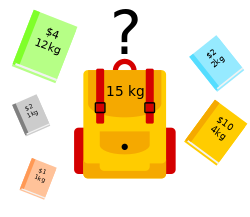
\includegraphics[width=0.5 \linewidth]{Knapsack_Problem_Illustration}
	\caption{Rucksackproblem anhand eines Beispiels \cite{VectorVoyager2023knapsack}}
	\label{fig:rucksackproblem}
\end{figure}

Das Problem ist NP-vollständig und kann mathematisch wie folgt formuliert werden:

Gegeben sei eine Menge $U$ von Objekten. Jedem Objekt $u \in U$ wird ein Gewicht $w(u)$ und ein Nutzenwert $v(u)$ zugeordnet. Es gibt außerdem eine Gewichtsschranke $B \in \mathbb{R}$.

Gesucht ist eine Teilmenge $K \subseteq U$, die die Bedingung

$$\sum_{u \in K} w(u) \leq B$$

einhält und die Zielfunktion

$$\sum_{u \in K} v(u)$$

maximiert. \cite{kellerer2004knapsack}

%********************************
% Komplexitätsanalyse
%********************************
\section{Komplexitätsanalyse}
Das Rucksackproblem gehört zur Komplexitätsklasse NP (nichtdeterministische Polynomialzeit). Dies bedeutet, dass das Problem mit einem deterministischen Algorithmus nicht in Polynomialzeit gelöst werden kann, sofern P ≠ NP. Eine Lösung in pseudopolynomialer Zeit kann jedoch z.B. mit Hilfe der dynamischen Programmierung gefunden werden. \cite{assi8672677}
Im Folgenden sollen nun drei Lösungsmöglichkeiten betrachtet werden.

%********************************
% Dynamisches Programmieren
%********************************
\newpage
\chapter{Dynamisches Programmieren}
Im ersten Schritt wird der Ansatz der dynamischen Programmierung betrachtet.
%********************************
% Prinzip des dynamischen Programmierens
%********************************
\section{Prinzip des dynamischen Programmierens}
Dynamische Programmierung basiert auf der Idee, ein Problem in kleinere Teilprobleme zu zerlegen und deren Lösungen zu speichern, um sie später wiederzuverwenden. Durch systematisches Kombinieren der Lösungen der Teilprobleme kann das Gesamtproblem effizient gelöst werden. Dieser Ansatz ist besonders nützlich bei Problemen mit überlappenden Teilstrukturen, bei denen viele Teilprobleme mehrfach auftreten. Die dynamische Programmierung ermöglicht eine optimale Lösung, indem es die Gesamtoptimalität aus lokalen optimalen Lösungen konstruiert wird.\cite{cormen2022introduction}

%********************************
%Iwas eigenes
%********************************
\section{Implementierung des dynamischen Programmierens für das Rucksackproblem}
\begin{algorithm}
	\caption{Dynamisches Programmieren für das Rucksackproblem}
	\begin{algorithmic}[1]
		\State \textbf{Input:} Liste von Gegenständen mit Gewicht $w_i$ und Wert $v_i$, maximales Gewicht $W$ des Rucksacks
		\State \textbf{Output:} Maximale Wertsumme, die in den Rucksack passt
		
		\State Initialisiere ein 2D-Array $dp$ mit Dimensionen $(n+1) \times (W+1)$ mit allen Einträgen auf $0$, wobei $n$ die Anzahl der Gegenstände ist
		
		\For{$i \gets 1$ to $n$}
		\For{$j \gets 0$ to $W$}
		\If{$w_i \leq j$}
		\State $dp[i][j] \gets \max(dp[i-1][j], dp[i-1][j-w_i] + v_i)$
		\Else
		\State $dp[i][j] \gets dp[i-1][j]$
		\EndIf
		\EndFor
		\EndFor
		
		\State \textbf{return} $dp[n][W]$
	\end{algorithmic}
\end{algorithm}


%********************************
%Iwas eigenes
%********************************
\section{Vor- und Nachteile}
\textbf{Vorteile:}
\begin{itemize}
	\item Optimale Lösungen: Es garantiert die optimale Lösung durch systematisches Durchsuchen aller möglichen Teilprobleme.
	\item Wiederverwendung von Teilproblemen: Durch das Speichern und Wiederverwenden von Lösungen für Teilprobleme werden redundante Berechnungen vermieden.
\end{itemize}

\textbf{Nachteile:}
\begin{itemize}
	\item Hoher Speicherbedarf: Erfordert eine große Menge an Speicherplatz, da Lösungen für alle Teilprobleme gespeichert werden müssen (Speicherkomplexität von $O(n \cdot W)$, wobei $n$ die Anzahl der Gegenstände und $W$ die Kapazität des Rucksacks ist).
	\item Nicht für große Eingaben geeignet: Bei sehr großen Problemen (z.B. sehr viele Gegenstände oder sehr große Kapazitäten) kann der Speicher- und Zeitbedarf trotz pseudopolynomialer Laufzeit sehr hoch sein.
\end{itemize}

%********************************
%Lösung
%********************************
\chapter{Greedy-Algorithmen}
Im Folgenden wird der Greedy-Algorithmus betrachtet.

%********************************
%Iwas eigenes
%********************************
\section{Prinzip der Greedy-Algorithmen}
Die Idee des Greedy-Algorithmus für das Rucksackproblem besteht darin, Elemente fortlaufend nach ihrer Gewichtsdichte \( c_j = \frac{a_j}{w_j} \) auszuwählen, solange die Kapazität des Rucksacks dies zulässt. Der Algorithmus beginnt mit einer Anfangslösung \( x = (0, \ldots, 0) \) und ersetzt schrittweise Nullen durch Einsen, und zwar in der Reihenfolge abnehmender Gewichtsdichte \( c_j \) (d.h. von den am besten geeigneten Elementen zu den am wenigsten geeigneten Elementen). Bei jedem Schritt wird überprüft, ob die neue Lösung noch machbar ist, d.h., ob die Gesamtgewichte die Kapazität des Rucksacks nicht überschreiten.

Der Prozess endet, wenn keine weiteren Elemente mehr hinzugefügt werden können, ohne die Kapazität zu überschreiten. Die so gefundene Lösung \( x_G \) wird als gierige Lösung bezeichnet. \cite{diubin2003average}

%Die Idee des Greedy Algorithmus für das Problem besteht in einer fortlaufenden Auswahl von Elementen mit der größten Gewichtsdichte cj=aj, solange die
%Rucksackkapazität dies zulässt. Formal gesehen beginnt der Algorithmus mit einer machbaren Lösung x ¼ ð0; ... ; 0Þ und ersetzt nacheinander Nullen durch Einsen in der
%Reihenfolge der abnehmenden Verhältnisse cj=aj (d.h. von links nach rechts);  jedes Mal wird die Machbarkeit der entsprechenden Lösung überprüft. Der Prozess wird beendet
%nachdem die letzte machbare Lösung gefunden wurde. Diese Lösung xG wird als gierige
%Lösung bezeichnet; der entsprechende Zielfunktionswert wird mit f G notiert. \cite{diubin2003average}

%********************************
%Iwas eigenes
%********************************
\section{Beispiele für Greedy-Lösungsansätze}
\begin{algorithm}
	\caption{Greedy-Algorithmus für das Rucksackproblem}
	\begin{algorithmic}[1]
		\State \textbf{Input:} Liste von Gegenständen mit Gewicht $w_i$ und Wert $v_i$, maximales Gewicht $W$ des Rucksacks
		\State \textbf{Output:} Liste von ausgewählten Gegenständen für den Rucksack
		
		\State Sortiere die Gegenstände absteigend nach dem Verhältnis $v_i/w_i$
		\State Initialisiere eine leere Liste $S$ für die ausgewählten Gegenstände
		\State Setze das aktuelle Gesamtgewicht $totalWeight$ des Rucksacks auf $0$
		
		\For{each Gegenstand $i$ in der sortierten Liste}
		\If{$totalWeight + w_i \leq W$}
		\State Füge den Gegenstand $i$ zu $S$ hinzu
		\State Erhöhe $totalWeight$ um $w_i$
		\EndIf
		\EndFor
		
		\State \textbf{return} $S$
	\end{algorithmic}
\end{algorithm}

%********************************
%Iwas eigenes
%********************************
\section{Vor- und Nachteile}
\textbf{Vorteile:} 
\begin{itemize}
	\item Effizienz: Hat eine kürzere Laufzeit (meist $O(nlogn)$ wegen des Sortierens), und ist daher bei großen Datensätzen schneller als dynamische Programmierung.
	\item Schnelle Entscheidungsfindung: Trifft schnelle Entscheidungen ohne Tracing, was die Ausführungszeit weiter verkürzt.
\end{itemize}

\textbf{Nachteile:}	
\begin{itemize}
	\item Keine optimale Lösung des Rucksackproblems: Führt nicht immer zu einer optimalen Lösung des klassischen Rucksackproblems.
	\item Eingeschränkte Flexibilität: Weniger flexibel bei der Anpassung an komplexere Variationen des Rucksackproblems im Vergleich zur dynamischen Programmierung.
\end{itemize}

%********************************
%Lösung
%********************************
\newpage
\chapter{First fit decreasing}
Es wird nun das Prinzip "First fit decreasing\dq \, betrachtet.
\section{Prinzip des First fit decreasing}
Der heuristische Ansatz \ac{FFD}, sortiert die Gegenstände absteigend nach ihrem Gewicht und legt jeden Gegenstand in den ersten Rucksack, in den er passt. Wird kein passender Rucksack gefunden, wird ein neuer Rucksack erstellt, und der Gegenstand wird in diesen eingefügt. Der \ac{FFD}-Algorithmus ist einfach zu implementieren und liefert in der Regel gute, wenn auch nicht optimale, Lösungen für das Rucksackproblem. \cite{martello1987algorithms}

\section{Beispiel für First fit decreasing}
\begin{algorithm}
	\caption{Heuristischer Ansatz "First-Fit-Decreasing" \, für das Rucksackproblem}
	\begin{algorithmic}[1]
		\State \textbf{Input:} Liste von Gegenständen mit Gewicht $w_i$ und Wert $v_i$, maximales Gewicht $W$ des Rucksacks
		\State \textbf{Output:} Liste von ausgewählten Gegenständen für den Rucksack
		
		\State Sortiere die Gegenstände absteigend nach dem Gewicht $w_i$
		\State Initialisiere eine Liste von Rucksäcken $B$ mit einem leeren Rucksack
		
		\For{each Gegenstand $i$ in der sortierten Liste}
		\State $j \gets 1$
		\While{$j \leq |B|$}
		\If{Gegenstand $i$ passt in Rucksack $B[j]$}
		\State Packe Gegenstand $i$ in Rucksack $B[j]$
		\State \textbf{break}
		\EndIf
		\State $j \gets j + 1$
		\EndWhile
		\If{kein passender Rucksack gefunden}
		\State Erstelle einen neuen Rucksack und packe Gegenstand $i$ hinein
		\State Füge den neuen Rucksack zu $B$ hinzu
		\EndIf
		\EndFor
		
		\State \textbf{return} Alle Gegenstände in den Rucksäcken in $B$
	\end{algorithmic}
\end{algorithm}

%********************************
%Iwas eigenes
%********************************
\section{Vor- und Nachteile}
\textbf{Vorteile:}
\begin{itemize}
	\item Schnelle Implementierung: Kann schnell implementiert werden, was es für einfache und schnelle Lösungsansätze attraktiv macht.
	\item Geringer Speicherbedarf: Benötigt neben den Eingabedaten nur wenig zusätzlichen Speicherplatz.
\end{itemize}

\textbf{Nachteile:}
\begin{itemize}
	\item Keine Garantie für optimale Lösungen: Liefert nicht immer die optimale Lösung, insbesondere bei komplexeren oder ungünstigeren Eingaben.
	\item Kann ineffizient sein: In einigen Fällen kann es zu einer schlechten Ausnutzung der Kapazität kommen, da Gegenstände früh platziert werden, ohne den zukünftigen Platzbedarf zu berücksichtigen.
\end{itemize}

\pagebreak
\chapter{Rucksackproblem in der Praxis}
	Im Folgenden werden die Anwendungsbereiche des Rucksackproblems sowie ein Beispiel für das Rucksackproblem dargestellt.
	
	\section{Anwendungsgebiete}
	Das Rucksackproblem findet in vielen Bereichen der realen Welt Anwendung. Hier einige Beispiele:
	
	\begin{itemize}
		\item \textbf{Ressourcenoptimierung:}
		\begin{itemize}
			\item \textbf{Zuschnitt von Rohmaterialien:} Das Rucksackproblem kann verwendet werden, um den Verschnitt beim Zuschnitt von Rohmaterialien zu minimieren.\cite{kellerer2004knapsack} 
			\item \textbf{Auswahl von Investitionen:} Das Rucksackproblem kann verwendet werden, um die optimale Auswahl von Investitionen für ein Portfolio zu finden.\cite{kellerer2004knapsack}
			\item \textbf{Auswahl von Vermögenswerten:} Das Rucksackproblem kann verwendet werden, um die optimale Auswahl von Vermögenswerten für eine Asset-Backed Securitization zu finden.\cite{kellerer2004knapsack}
		\end{itemize}
		\item \textbf{Kryptographie:}
		\begin{itemize}
			\item \textbf{Generierung von Schlüsseln:} Das Rucksackproblem kann verwendet werden, um Schlüssel für kryptographische Systeme wie das Merkle-Hellman-Kryptosystem zu generieren.\cite{kellerer2004knapsack}
		\end{itemize}
	\end{itemize}


	\section{Beispiel}
		Es folgt ein Beispiel für den Greedy-Algortihmus.
	
		\subsection{Problemstellung}
		Ein Kobold steht vor einem Dilemma: Eine Schatzkammer voller wertvoller Gegenstände, aber in seinem Rucksack ist nur begrenzt Platz. Wie kann er seinen Gewinn maximieren, ohne zu viel Gewicht zu tragen?
		
		Rucksackkapazität des Kobolds: 5kg \\
		Verfügbare Gegenstände \ref{tab:Preis und Gewichtsverhältnisse der Gegenstände}:      
		\begin{table}[H]
			\begin{center}
				\begin{adjustbox}{width=\columnwidth,center}
					\begin{tabular}{|c|c|c|c|}
						\hline
						Name & Preis (Gold) & Gewicht (kg) & Preis/Gewicht (Gold/kg)
						\\
						\hline
						Glücksbringer & 125 & 0,25 & 500
						\\
						\hline
						Opalglitzerschmuck & 150 & 0,5 & 300
						\\
						\hline
						Amethystkette & 60 & 0,25 & 240
						\\
						\hline
						Glühender Rubin & 200 & 1 & 200
						\\
						\hline
						Mystischer Aquamarin & 300 & 2 & 150
						\\
						\hline
						Säckchen Goldmünzen & 50 & 0,5 & 100
						\\
						\hline
						Kugel des Untergangs & 70 & 1 & 70
						\\
						\hline
						Antiker Elfenring & 50 & 1 & 50
						\\
						\hline
						Handvoll Kupferstücke & 10 & 0,5 & 20
						\\
						\hline
						Silberbarren & 20 & 2 & 10
						\\
						\hline
					\end{tabular} 
				\end{adjustbox}
			\end{center} 
			\caption{Preis und Gewichtsverhältnisse der Gegenstände}
			\label{tab:Preis und Gewichtsverhältnisse der Gegenstände}
		\end{table}
		
		\subsection{Lösung des Beispiels}
		Typisch für seine Art verwendet der Kobold für dieses Problem den Greedy-Algorithmus. Er nimmt also die Gegenstände mit dem höchsten Wert pro Gewicht, solange sie noch in seinen Rucksack passen. 
		Vom Glücksbringer bis einschließlich zum Säckchen Goldmünzen passen alle Gegenstände in den Rucksack. Danach kann der Kobold weder die Kugel des Untergangs noch den antiken Elfenring mitnehmen und nimmt stattdessen noch die Handvoll Kupferstücke mit. Damit erreicht der Kobold 895 Gold mit 5kg Gewicht. 
	
		\subsection{Diskussion der Ergebnisse}
		Der Greedy-Ansatz weicht hier nur unwesentlich von der besten Lösung ab, bei der der Kobold statt der Handvoll Kupferstücke und dem Säckchen Goldmünzen die Kugel des Untergangs mitnehmen sollte, für insgesamt 905 Gold. Der Greedy-Alogithmus liefert, wie man sieht, nicht immer die beste Lösung, aber eine gute Annäherung in sehr kurzer Zeit.

%********************************
%Zusammenfassung und Ausblick
%********************************
\newpage
\chapter{Zusammenfassung und Ausblick}
Das Rucksackproblem ist ein grundlegendes Optimierungsproblem der Informatik und Mathematik mit einem breiten Anwendungsspektrum. Trotz seiner scheinbaren Einfachheit ist das Problem aufgrund seiner exponentiellen Komplexität eine Herausforderung. Es gibt verschiedene Lösungsansätze, z.B. die dynamische Programmierung, der Greedy-Algorithmus oder das First-Fit-Descreasing, das zwar eine Lösung in pseudopolynomialer Zeit liefert, aber nicht immer korrekt ist. Die vorgestellten Ansätze bieten verschiedene Herangehensweisen an das Rucksackproblem, aber es gibt noch Raum für weitere Untersuchungen und Verbesserungen. Die Integration von Techniken des Machine-Learning könnte neue Möglichkeiten zur Lösung des Rucksackproblems eröffnen und gleichzeitig den steigenden Anforderungen in verschiedenen Anwendungsbereichen gerecht werden.

%********************************
%Literaturverzeichnis
%********************************
\newpage
\pagenumbering{Roman}
\setcounter{page}{\value{frontmatterPage}} %Bei \pagenumbering wird Seitenzähler zurückgesetzt, hier wird der gespeicherte Wert vom frontmatter weitergeführt
\addtocounter{page}{1}
\addcontentsline{toc}{chapter}{\protect\numberline{}Literaturverzeichnis}

%Quellenverzeichnis
\renewcommand{\refname}{Literaturverzeichnis}
\bibliographystyle{IEEEtran}
\bibliography{./sources}


\end{document}
